Este apêndice reúne, para os blocos menores do projeto digital, a visão RTL gerada pelo Quartus e as formas de onda dos \eng{testbenches} correspondentes. Todos os \eng{testbenches} terminaram sem erros (Tabela~\ref{tab:testbenches}).

\section{Somador}

O somador (\cod{word\_adder}) é um único somador de 32~bits, \cod{Add0}, sem vai-um de entrada (Figura~\ref{fig:rtl_add}). A Figura~\ref{fig:tb_add} mostra os casos de borda do \eng{testbench}, incluindo o estouro: \cod{FFFFFFFF} mais 1 resulta em zero, e \cod{80000000} mais \cod{80000000} também.

\begin{figure}
	\caption{Visão RTL do somador (\cod{word\_adder}).}
	\label{fig:rtl_add}
	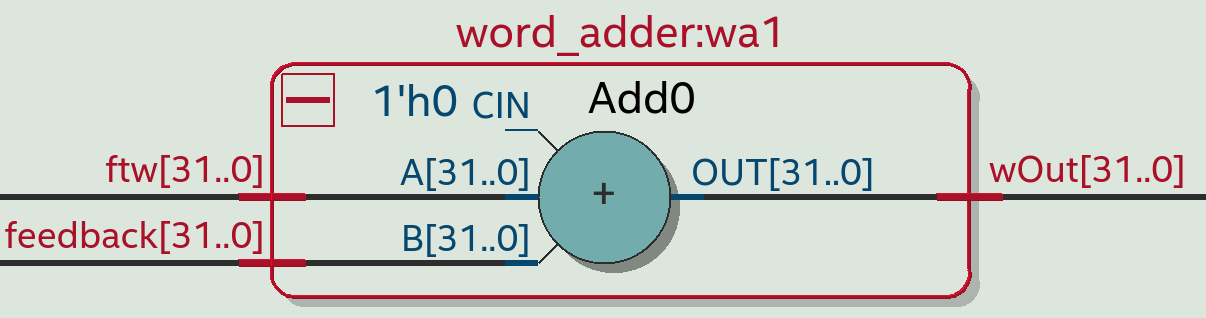
\includegraphics[width=0.8\textwidth]{./figuras/rtl_word_adder}
	\legend{Fonte~---~Autoria própria.}
\end{figure}

\begin{figure}
	\caption{Casos de borda do somador.}
	\label{fig:tb_add}
	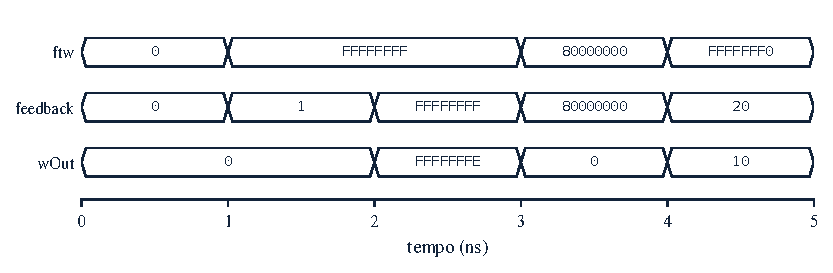
\includegraphics[width=\textwidth]{./figuras/tb_word_adder}
	\legend{Fonte~---~Autoria própria.}
\end{figure}

\section{Registrador de fase}

O registrador de fase (\cod{phase\_register}) é um registrador de 32~bits com \eng{reset} assíncrono, ligado à entrada CLRN (Figura~\ref{fig:rtl_preg}). A Figura~\ref{fig:tb_preg} mostra a carga na borda de subida e o \eng{reset} no meio de um ciclo, que zera a saída imediatamente.

\begin{figure}
	\caption{Visão RTL do registrador de fase (\cod{phase\_register}).}
	\label{fig:rtl_preg}
	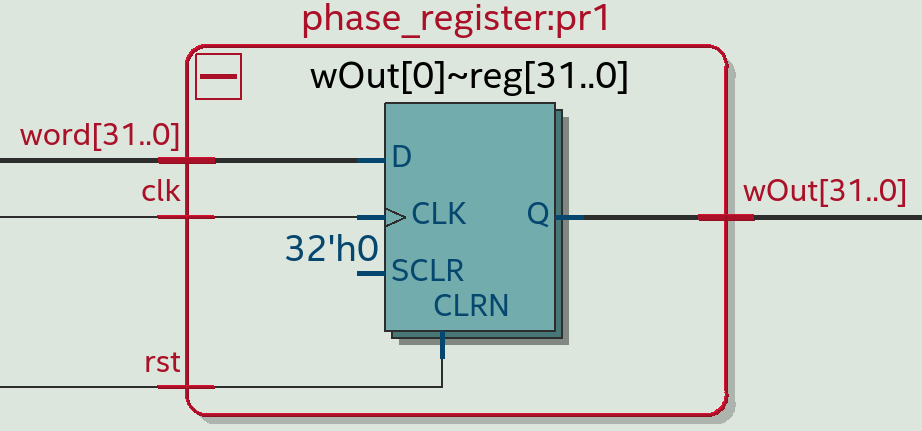
\includegraphics[width=0.7\textwidth]{./figuras/rtl_phase_register}
	\legend{Fonte~---~Autoria própria.}
\end{figure}

\begin{figure}
	\caption{Registrador de fase: acima, a saída do \eng{reset} e as cargas; abaixo, o \eng{reset} assíncrono.}
	\label{fig:tb_preg}
	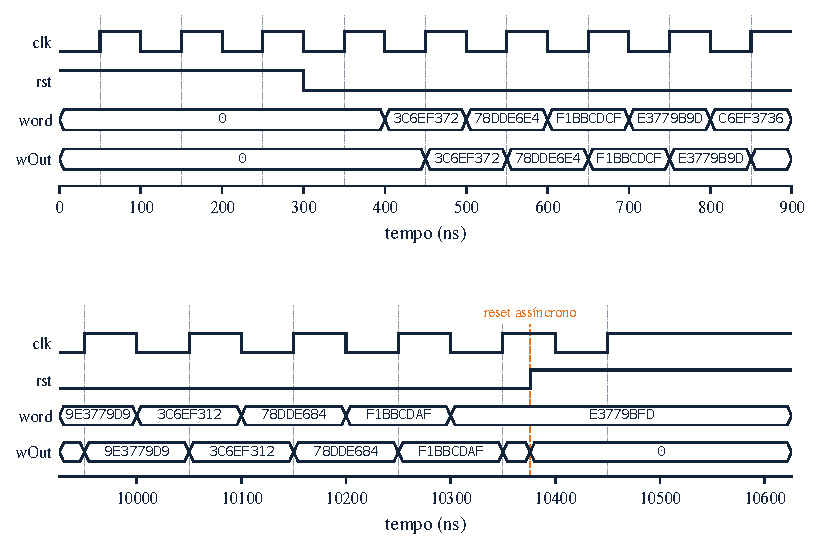
\includegraphics[width=\textwidth]{./figuras/tb_phase_register}
	\legend{Fonte~---~Autoria própria.}
\end{figure}

\section{Truncador}

O truncador (\cod{truncator}) não tem lógica: a visão RTL (Figura~\ref{fig:rtl_trunc}) mostra apenas a ligação dos bits 31 a 22 da fase à saída. A Figura~\ref{fig:tb_trunc} mostra os casos de borda, como a fase \cod{3FFFFF}, último valor do endereço 0, e \cod{400000}, primeiro do endereço 1.

\begin{figure}
	\caption{Visão RTL do truncador (\cod{truncator}).}
	\label{fig:rtl_trunc}
	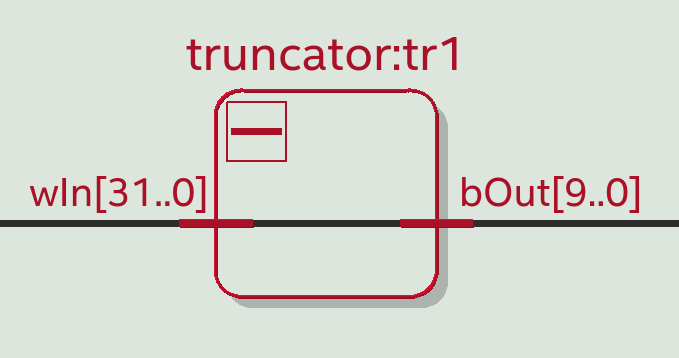
\includegraphics[width=0.5\textwidth]{./figuras/rtl_truncator}
	\legend{Fonte~---~Autoria própria.}
\end{figure}

\begin{figure}
	\caption{Casos de borda do truncador.}
	\label{fig:tb_trunc}
	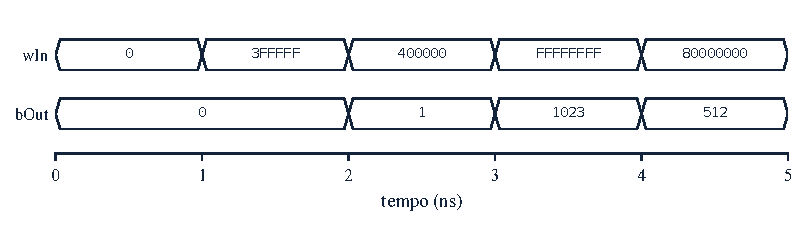
\includegraphics[width=\textwidth]{./figuras/tb_truncator}
	\legend{Fonte~---~Autoria própria.}
\end{figure}

\section{Multiplexador de saída}

O multiplexador de saída (\cod{out\_mux}) foi inferido como oito multiplexadores de quatro entradas, um por bit, todos controlados por \cod{sel} (Figura~\ref{fig:rtl_mux}). A Figura~\ref{fig:tb_mux} mostra a saída seguindo a entrada escolhida para cada código.

\begin{figure}
	\caption{Visão RTL do multiplexador de saída (\cod{out\_mux}).}
	\label{fig:rtl_mux}
	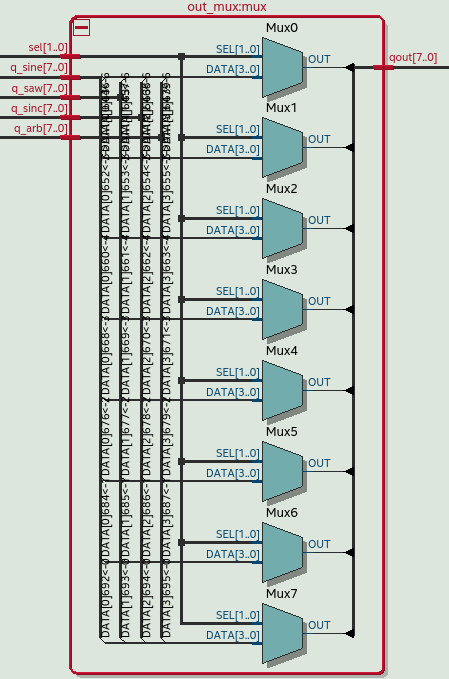
\includegraphics[width=0.45\textwidth]{./figuras/rtl_out_mux}
	\legend{Fonte~---~Autoria própria.}
\end{figure}

\begin{figure}
	\caption{Seleção da forma de onda no multiplexador de saída.}
	\label{fig:tb_mux}
	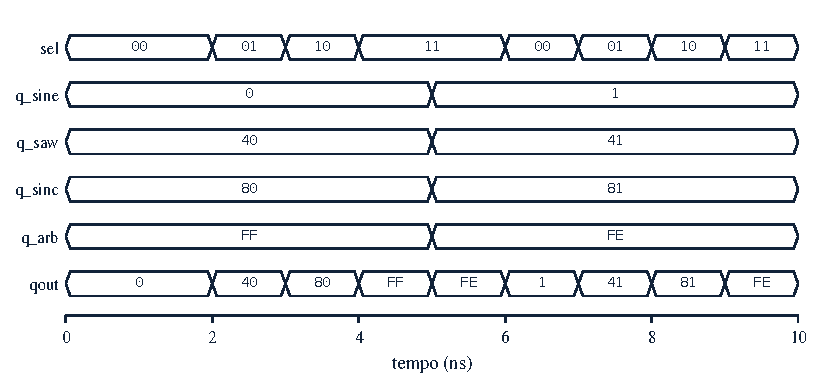
\includegraphics[width=\textwidth]{./figuras/tb_out_mux}
	\legend{Fonte~---~Autoria própria.}
\end{figure}

\section{Registrador de saída}

O registrador de saída (\cod{output\_register}) deve assumir o código 128 (\cod{80} em hexadecimal) no \eng{reset}. A visão RTL (Figura~\ref{fig:rtl_oreg}) mostra como isso foi inferido: os bits 0 a 6 usam a entrada de \eng{clear} (CLRN), e o bit 7, a de \eng{preset} (PRE). A Figura~\ref{fig:tb_oreg} mostra a saída em \cod{80} durante o \eng{reset} e as cargas seguintes.

\begin{figure}
	\caption{Visão RTL do registrador de saída (\cod{output\_register}).}
	\label{fig:rtl_oreg}
	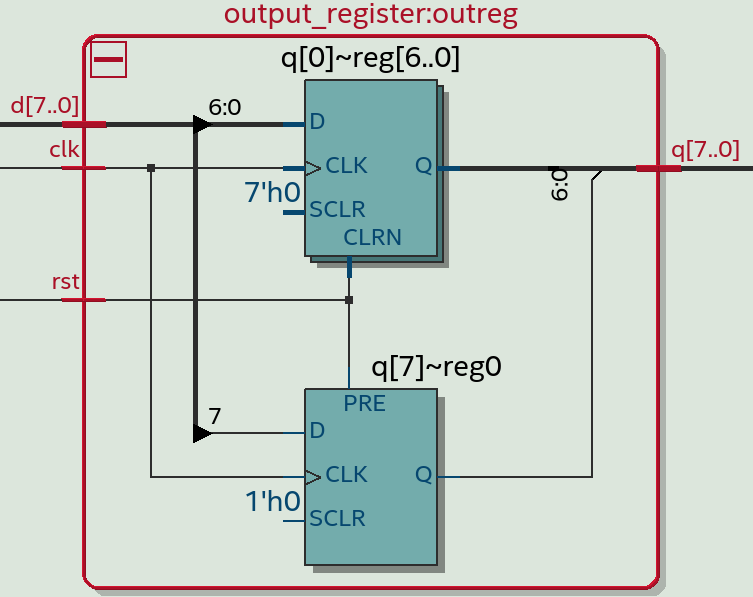
\includegraphics[width=0.65\textwidth]{./figuras/rtl_output_register}
	\legend{Fonte~---~Autoria própria.}
\end{figure}

\begin{figure}
	\caption{Registrador de saída: código 128 no \eng{reset} e carga na borda.}
	\label{fig:tb_oreg}
	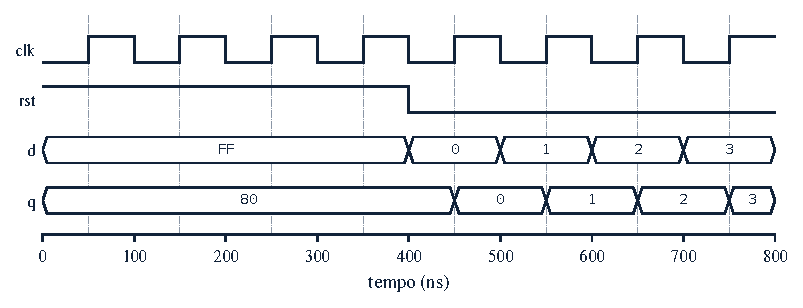
\includegraphics[width=\textwidth]{./figuras/tb_output_register}
	\legend{Fonte~---~Autoria própria.}
\end{figure}

\section{Sincronizador de reset}

O sincronizador de \eng{reset} (\cod{reset\_sync}) é uma cadeia de três \eng{flip-flops} (\cod{chain}) com \eng{preset} assíncrono, que desloca zeros a cada clock (Figura~\ref{fig:rtl_rsync}). A Figura~\ref{fig:tb_rsync} mostra a entrada em \eng{reset} no instante em que \cod{rst\_in} sobe e a saída na terceira borda depois de \cod{rst\_in} cair.

\begin{figure}
	\caption{Visão RTL do sincronizador de \eng{reset} (\cod{reset\_sync}).}
	\label{fig:rtl_rsync}
	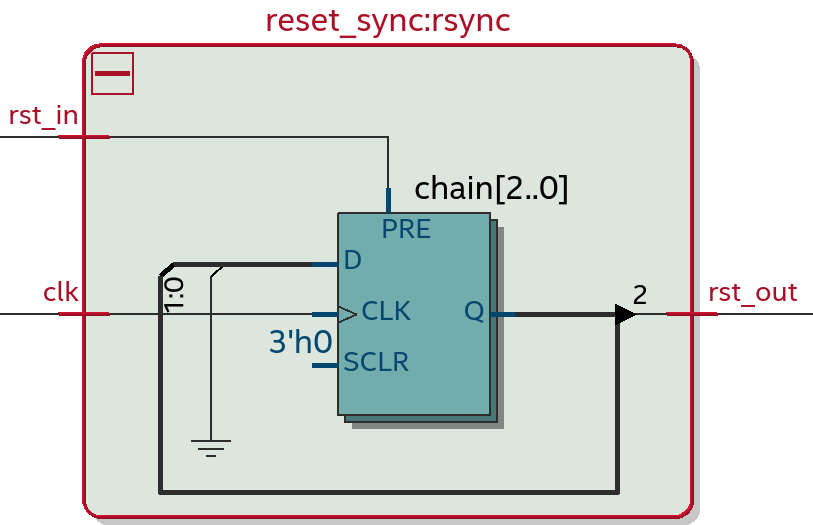
\includegraphics[width=0.65\textwidth]{./figuras/rtl_reset_sync}
	\legend{Fonte~---~Autoria própria.}
\end{figure}

\begin{figure}
	\caption{Entrada e saída do \eng{reset} no sincronizador.}
	\label{fig:tb_rsync}
	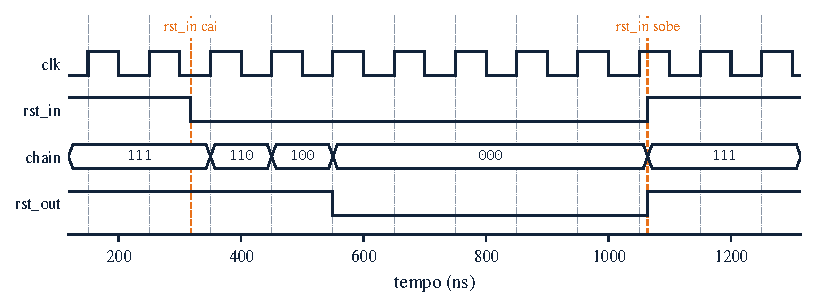
\includegraphics[width=\textwidth]{./figuras/tb_reset_sync}
	\legend{Fonte~---~Autoria própria.}
\end{figure}

\section{Registradores de controle}

A Figura~\ref{fig:rtl_regs} mostra os registradores de controle (\cod{control\_registers}) no RTL: (a) as portas do bloco e (b) a lógica interna, com os registradores de configuração e os multiplexadores que os atualizam conforme a instrução. A Figura~\ref{fig:tb_regs} mostra a decodificação dos primeiros comandos do \eng{testbench}: frequência, forma de onda e escritas na tabela, cada uma com um pulso de um clock em \cod{lut\_we}.

\begin{figure}
	\caption{Visão RTL dos registradores de controle (\cod{control\_registers}): (a) portas do bloco; (b) lógica interna.}
	\label{fig:rtl_regs}
	\begin{minipage}[b]{0.62\textwidth}
		\centering
		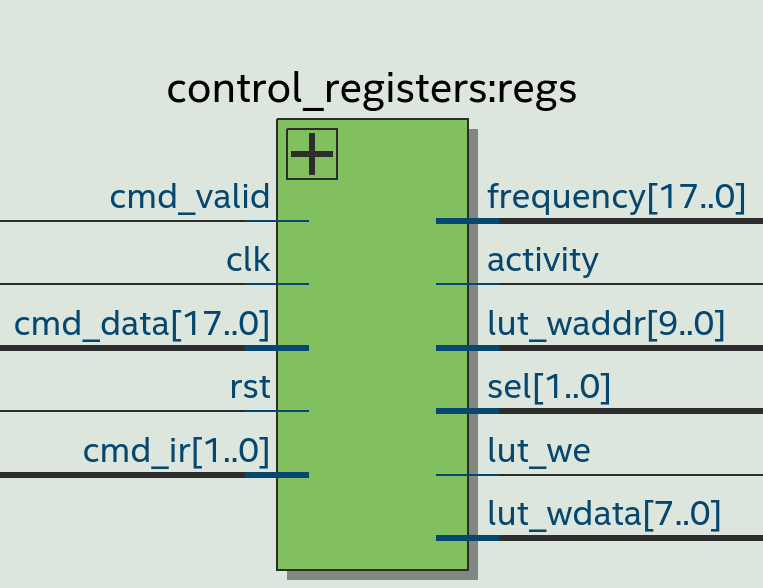
\includegraphics[height=6.5cm]{./figuras/rtl_control_registers_2}\\[2pt]
		{\smallfont (a)}
	\end{minipage}%
	\hfill
	\begin{minipage}[b]{0.34\textwidth}
		\centering
		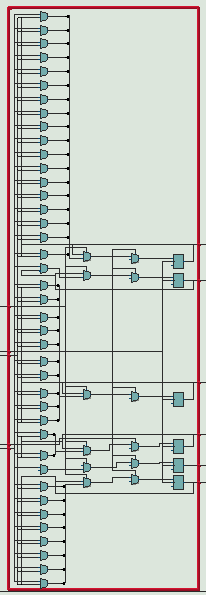
\includegraphics[height=6.5cm]{./figuras/rtl_control_registers_1}\\[2pt]
		{\smallfont (b)}
	\end{minipage}
	\legend{Fonte~---~Autoria própria.}
\end{figure}

\begin{figure}
	\caption{Decodificação dos comandos nos registradores de controle.}
	\label{fig:tb_regs}
	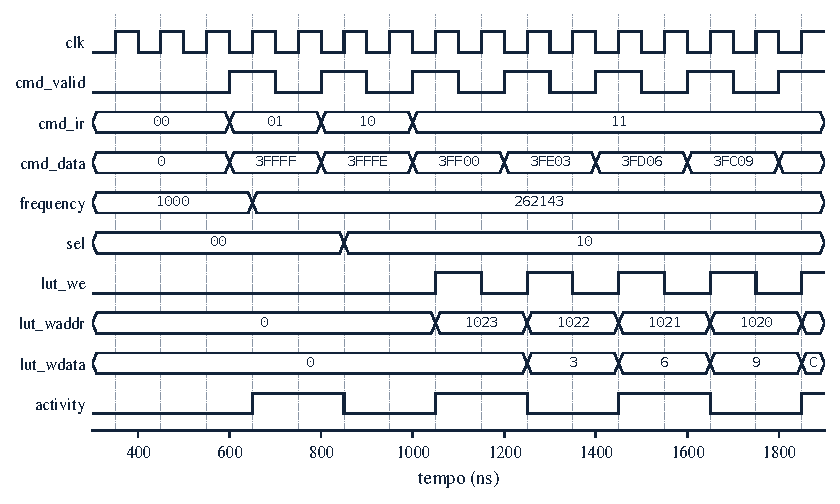
\includegraphics[width=\textwidth]{./figuras/tb_control_registers}
	\legend{Fonte~---~Autoria própria.}
\end{figure}
